\documentclass[12pt]{article}
\usepackage[margin=1in]{geometry}
\usepackage{amsmath}
\usepackage{amssymb}
\usepackage{tikz}
\usepackage{pgfplots}
\usepackage{mdframed}
\usepackage{xcolor}
\usepackage{enumitem}
\usepackage{multicol}
\usepackage{array}
\usepackage[T1]{fontenc}
\usepackage{inputenc}
\usepackage{parskip}

\pgfplotsset{compat=1.18}
\usetikzlibrary{arrows.meta, decorations.pathmorphing}

% ── Colour palette ──────────────────────────────────────────────────────────
\definecolor{minionYellow}{RGB}{240, 195, 0}
\definecolor{minionBlue}{RGB}{50, 100, 180}
\definecolor{skyBlue}{RGB}{220, 235, 255}
\definecolor{grassGreen}{RGB}{60, 160, 60}
\definecolor{lightGray}{RGB}{245, 245, 245}
\definecolor{hintGray}{RGB}{130, 130, 130}

% ── Framed environments ─────────────────────────────────────────────────────
\newmdenv[
  backgroundcolor=skyBlue,
  linecolor=minionBlue,
  linewidth=2pt,
  roundcorner=6pt,
  innertopmargin=10pt,
  innerbottommargin=10pt,
  innerleftmargin=12pt,
  innerrightmargin=12pt,
]{conceptbox}

\newmdenv[
  backgroundcolor=minionYellow!25,
  linecolor=minionYellow!70!black,
  linewidth=2pt,
  roundcorner=6pt,
  innertopmargin=10pt,
  innerbottommargin=10pt,
  innerleftmargin=12pt,
  innerrightmargin=12pt,
]{warningbox}

\newmdenv[
  backgroundcolor=lightGray,
  linecolor=gray!50,
  linewidth=1pt,
  roundcorner=4pt,
  innertopmargin=6pt,
  innerbottommargin=6pt,
]{workbox}

% ── Answer blank ─────────────────────────────────────────────────────────────
\newcommand{\blank}[1][4cm]{\underline{\hspace{#1}}}

\setlength{\parskip}{6pt}
\setlength{\parindent}{0pt}

% ─────────────────────────────────────────────────────────────────────────────
\begin{document}

% ── Header ───────────────────────────────────────────────────────────────────
\begin{center}
  {\LARGE\bfseries\color{minionBlue} Minion Catapult: Algebra Unlocked!}\\[6pt]
  {\large Name: \blank[7cm] \quad Date: \blank[3cm]}\\[4pt]
  {\normalsize\color{hintGray}
    Algebra isn't just symbols --- it's a cheat code for answering questions
    \emph{without} guessing.}
\end{center}

\vspace{6pt}\noindent\rule{\linewidth}{1pt}\vspace{6pt}

% ═══════════════════════════════════════════════════════════════════════════
\section*{Background: The Flight Formula}
% ═══════════════════════════════════════════════════════════════════════════

When the minion is launched from the catapult, the simulation displays an
equation that describes the entire flight path:

\[
  h \;=\; A\,d^2 \;+\; B\,d
\]

\begin{itemize}
  \item $d$ = horizontal distance (meters) from the catapult
  \item $h$ = height (meters) above the ground
  \item $A$ and $B$ are numbers the simulator calculates from your launch
        speed and angle
\end{itemize}

This kind of equation --- a \textbf{quadratic} --- always makes a U-shape
(or arch shape) called a \textbf{parabola}.  The minion follows the top half
of that arch.

\begin{center}
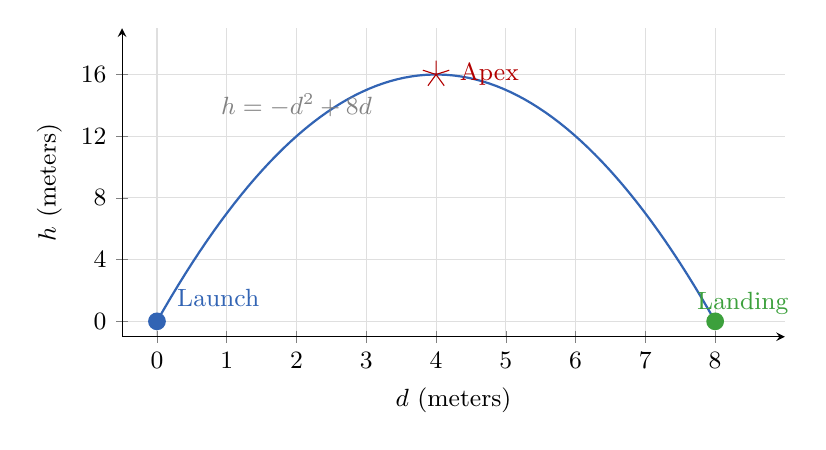
\begin{tikzpicture}
  \begin{axis}[
    width=10cm, height=5.5cm,
    xmin=-0.5, xmax=9,
    ymin=-1, ymax=19,
    axis lines=left,
    xlabel={$d$ (meters)},
    ylabel={$h$ (meters)},
    xtick={0,1,...,8},
    ytick={0,4,8,12,16},
    tick label style={font=\small},
    label style={font=\small},
    grid=major,
    grid style={gray!25},
    clip=false,
  ]
    % Parabola h = -x^2 + 8x
    \addplot[thick, minionBlue, domain=0:8, samples=80] {-x^2 + 8*x};
    % Launch point
    \addplot[only marks, mark=*, mark size=3pt, minionBlue] coordinates {(0,0)};
    % Landing point
    \addplot[only marks, mark=*, mark size=3pt, grassGreen] coordinates {(8,0)};
    % Apex
    \addplot[only marks, mark=star, mark size=5pt, red!70!black] coordinates {(4,16)};
    % Labels
    \node[font=\small, minionBlue, right] at (axis cs:0.15, 1.5) {Launch};
    \node[font=\small, grassGreen, right] at (axis cs:7.6, 1.2) {Landing};
    \node[font=\small, red!70!black, right] at (axis cs:4.2, 16) {Apex};
    % Equation label
    \node[font=\small\itshape, hintGray] at (axis cs:2, 14) {$h = -d^2 + 8d$};
  \end{axis}
\end{tikzpicture}
\end{center}

% ═══════════════════════════════════════════════════════════════════════════
\section*{Part 1 \quad Factoring the Formula --- Find the Landing Spot}
% ═══════════════════════════════════════════════════════════════════════════

\begin{conceptbox}
\textbf{Big Idea:} The minion is on the ground whenever $h = 0$.  Set the
formula equal to zero and solve for $d$.  Factoring lets you do this
\emph{instantly} --- no guessing required!

\medskip
\textbf{Factoring trick for $h = Ad^2 + Bd$:} \;
Pull out the common factor of $d$:
\[
  Ad^2 + Bd \;=\; d\,(Ad + B) \;=\; 0
\]
A product equals zero when \emph{at least one factor is zero}, so:
\[
  d = 0 \quad (\text{launch point}) \qquad \text{or} \qquad Ad + B = 0
  \;\Rightarrow\; d = -\tfrac{B}{A} \quad (\text{landing point})
\]
\end{conceptbox}

\subsection*{Worked Example}

Suppose the simulator shows: \quad $h = -d^2 + 8d$

\textbf{Step 1 --- Factor:}
\[
  h = d(-d + 8)
\]

\textbf{Step 2 --- Set $h = 0$ and solve:}
\[
  d = 0 \qquad \text{or} \qquad -d + 8 = 0 \;\Rightarrow\; d = 8
\]

\textbf{Conclusion:} The minion launches at $d = 0$\,m and lands at
$\boxed{d = 8}$\,m.  Done --- no trial and error!

\bigskip
\textbf{Practice Problems}

\begin{enumerate}[leftmargin=*, label=\textbf{\arabic*.}]

\item The simulator shows $h = -2d^2 + 12d$.

  \begin{workbox}
  Factor: \quad $h = $ \blank[7cm] \\[10pt]
  Set $h = 0$: \quad $d = 0 \quad$ or $\quad d = $ \blank[2.5cm]\\[10pt]
  The minion lands at $d = $ \blank[2cm] meters.
  \end{workbox}

\vspace{8pt}
\item The simulator shows $h = -3d^2 + 15d$.

  \begin{workbox}
  Factor: \quad $h = $ \blank[7cm] \\[10pt]
  Set $h = 0$: \quad $d = 0 \quad$ or $\quad d = $ \blank[2.5cm]\\[10pt]
  The minion lands at $d = $ \blank[2cm] meters.
  \end{workbox}

\vspace{8pt}
\item The simulator shows $h = -0.5d^2 + 6d$.

  \begin{workbox}
  Factor: \quad $h = $ \blank[7cm] \\[10pt]
  Set $h = 0$: \quad $d = $ \blank[2cm] or $d = $ \blank[2cm]\\[10pt]
  The minion lands at $d = $ \blank[2cm] meters.
  \end{workbox}

\vspace{8pt}
\item \textbf{Challenge:} The simulator shows $h = -\tfrac{1}{4}d^2 + 5d$.
      Factor and find the landing distance.

  \begin{workbox}
  \vspace{2.5cm}
  The minion lands at $d = $ \blank[2cm] meters.
  \end{workbox}

\end{enumerate}

\newpage

% ═══════════════════════════════════════════════════════════════════════════
\section*{Part 2 \quad Finding the Apex --- The Highest Point}
% ═══════════════════════════════════════════════════════════════════════════

\begin{conceptbox}
\textbf{Big Idea:} A parabola is perfectly symmetric.  The highest point
(apex) is always directly \emph{above the midpoint} between the two roots.

\medskip
\textbf{Two-step method:}
\begin{enumerate}[nosep]
  \item Find the two roots (where $h = 0$).  You already know how!
  \item Average them: \quad
        $d_{\text{apex}} = \dfrac{d_1 + d_2}{2}$
  \item Plug $d_{\text{apex}}$ back into the formula to get
        $h_{\text{apex}}$.
\end{enumerate}
\end{conceptbox}

\subsection*{Worked Example}

Formula: $h = -d^2 + 8d$

\textbf{Step 1 --- Roots:} $d = 0$ and $d = 8$ (from Part 1).

\textbf{Step 2 --- Midpoint:}
\[
  d_{\text{apex}} = \frac{0 + 8}{2} = 4
\]

\textbf{Step 3 --- Height at apex:}
\[
  h_{\text{apex}} = -(4)^2 + 8(4) = -16 + 32 = \boxed{16 \text{ meters}}
\]

The apex is at the point $(4, 16)$: four meters out, sixteen meters up.

\bigskip
\textbf{Practice Problems}

\begin{enumerate}[leftmargin=*, label=\textbf{\arabic*.}, resume]

\item Find the apex of $h = -2d^2 + 12d$.

  \begin{workbox}
  Roots: $d = $ \blank[2cm] and $d = $ \blank[2cm] \\[10pt]
  Midpoint: $d_{\text{apex}} = \dfrac{\blank[1.5cm] + \blank[1.5cm]}{2}
  = $ \blank[1.5cm] \\[10pt]
  Height: $h_{\text{apex}} = $ \blank[6cm] $= $ \blank[1.5cm] meters\\[10pt]
  Apex point: $\bigl($ \blank[1cm] , \blank[1cm] $\bigr)$
  \end{workbox}

\vspace{8pt}
\item Find the apex of $h = -3d^2 + 15d$.

  \begin{workbox}
  Roots: \blank[2cm] and \blank[2cm] \quad
  Midpoint: \blank[2cm] \\[10pt]
  Height: \blank[8cm] \\[10pt]
  Apex point: $\bigl($ \blank[1cm] , \blank[1cm] $\bigr)$
  \end{workbox}

\vspace{8pt}
\item \textbf{Think about it:} In Problem~5, which is larger --- the landing
  distance or twice the apex $d$-value?  Why does that make sense given the
  symmetry of a parabola?

  \begin{workbox}
  \vspace{2cm}
  \end{workbox}

\end{enumerate}

% ═══════════════════════════════════════════════════════════════════════════
\section*{Part 3 \quad Other Quadratics --- ``Trinomials''}
% ═══════════════════════════════════════════════════════════════════════════

\begin{conceptbox}
Not every quadratic is a catapult formula.  Some have three terms:
\[
  y = x^2 + bx + c
\]
To factor these, find two numbers that \textbf{multiply to $c$} and
\textbf{add to $b$}:
\[
  x^2 + bx + c = (x + p)(x + q)
  \qquad \text{where } p \cdot q = c \text{ and } p + q = b
\]
The roots (where $y = 0$) are then $x = -p$ and $x = -q$.
\end{conceptbox}

\subsection*{Worked Example}

Factor $y = x^2 + 5x + 6$.

\textit{Find two numbers that multiply to 6 and add to 5.}

\medskip
\begin{center}
\begin{tabular}{c|c|c}
\textbf{Pairs that multiply to 6} & \textbf{Their sum} & \textbf{Match?}\\
\hline
$1 \times 6$ & $7$ & No\\
$2 \times 3$ & $5$ & \textbf{Yes!}\\
\end{tabular}
\end{center}

\medskip
So $y = (x + 2)(x + 3)$, and the roots are $x = -2$ and $x = -3$.

\bigskip
\textbf{Practice Problems}

\begin{enumerate}[leftmargin=*, label=\textbf{\arabic*.}, resume]

\item Factor $y = x^2 + 7x + 12$.

  \textit{Find two numbers: multiply to} \blank[1.5cm], \textit{add to} \blank[1.5cm].

  \begin{workbox}
  Numbers: \blank[1.5cm] and \blank[1.5cm] \\[10pt]
  Factored: $y = (x + \blank[1cm])(x + \blank[1cm])$ \\[10pt]
  Roots: $x = $ \blank[1.5cm] and $x = $ \blank[1.5cm]
  \end{workbox}

\vspace{8pt}
\item Factor $y = x^2 - 6x + 8$.

  \textit{Hint: since $b$ is negative and $c$ is positive, both numbers are negative.}

  \begin{workbox}
  Numbers: \blank[1.5cm] and \blank[1.5cm] \\[10pt]
  Factored: $y = (x - \blank[1cm])(x - \blank[1cm])$ \\[10pt]
  Roots: $x = $ \blank[1.5cm] and $x = $ \blank[1.5cm]
  \end{workbox}

\vspace{8pt}
\item Factor $y = x^2 - x - 6$.

  \textit{Hint: since $c$ is negative, one number is positive and one is negative.}

  \begin{workbox}
  Numbers that multiply to $-6$ and add to $-1$: \blank[1.5cm] and \blank[1.5cm] \\[10pt]
  Factored: $y = (x + \blank[1cm])(x - \blank[1cm])$ \\[10pt]
  Roots: $x = $ \blank[1.5cm] and $x = $ \blank[1.5cm]
  \end{workbox}

\vspace{8pt}
\item Factor and find the roots of $y = x^2 + 2x - 15$.

  \begin{workbox}
  \vspace{2.5cm}
  Roots: $x = $ \blank[1.5cm] and $x = $ \blank[1.5cm]
  \end{workbox}

\end{enumerate}

\newpage

% ═══════════════════════════════════════════════════════════════════════════
\section*{Part 4 \quad The Axis of Symmetry and Vertex (Trinomials)}
% ═══════════════════════════════════════════════════════════════════════════

\begin{conceptbox}
The same midpoint trick works for \emph{any} quadratic, not just catapult
formulas.  Once you have the roots, average them to find the
\textbf{axis of symmetry} (the vertical line through the top or bottom of
the parabola), then plug in to find the \textbf{vertex}.

\medskip
When $y = x^2 + bx + c$ (positive $x^2$ term), the parabola opens
\textbf{upward}, so the vertex is the \textbf{minimum} point.
\end{conceptbox}

\subsection*{Worked Example}

$y = x^2 + 5x + 6 = (x+2)(x+3)$. \quad Roots: $x = -2$ and $x = -3$.

\[
  x_{\text{vertex}} = \frac{-2 + (-3)}{2} = \frac{-5}{2} = -2.5
\]

\[
  y_{\text{vertex}} = (-2.5)^2 + 5(-2.5) + 6 = 6.25 - 12.5 + 6 = -0.25
\]

Vertex: $(-2.5,\ -0.25)$ --- the lowest point of this parabola.

\bigskip
\textbf{Practice Problems}

\begin{enumerate}[leftmargin=*, label=\textbf{\arabic*.}, resume]

\item For $y = x^2 - 6x + 8$, find the vertex.

  \begin{workbox}
  Roots (from Problem~9): $x = $ \blank[1.5cm] and $x = $ \blank[1.5cm] \\[10pt]
  Axis of symmetry: $x_v = \dfrac{\blank[1.5cm] + \blank[1.5cm]}{2} = $ \blank[1.5cm] \\[10pt]
  $y_v = $ \blank[8cm] $= $ \blank[1.5cm] \\[10pt]
  Vertex: $\bigl($ \blank[1cm] , \blank[1cm] $\bigr)$
  \end{workbox}

\vspace{8pt}
\item Without graphing, does $y = x^2 + 2x - 15$ have a maximum or a minimum?
  How do you know?  Find the vertex.

  \begin{workbox}
  Max or min? \blank[3cm] \quad Because: \blank[6cm] \\[10pt]
  Roots (from Problem~12): $x = $ \blank[1.5cm] and $x = $ \blank[1.5cm] \\[10pt]
  Vertex: \blank[8cm]
  \end{workbox}

\end{enumerate}

% ═══════════════════════════════════════════════════════════════════════════
\section*{Part 5 \quad Challenge Problems}
% ═══════════════════════════════════════════════════════════════════════════

\begin{enumerate}[leftmargin=*, label=\textbf{\arabic*.}, resume]

\item A minion is launched and the simulator shows $h = -d^2 + 10d$.

  \begin{enumerate}[label=(\alph*)]
    \item Where does the minion land? \blank[3cm] meters

    \vspace{4pt}
    \item What is the maximum height? \blank[3cm] meters

    \vspace{4pt}
    \item At what distance does the minion reach its peak? \blank[3cm] meters
  \end{enumerate}

  \begin{workbox}
  \vspace{3cm}
  \end{workbox}

\vspace{8pt}
\item Two different minions are launched.  Minion~A has formula
  $h = -d^2 + 8d$ and Minion~B has formula $h = -d^2 + 10d$.
  \begin{enumerate}[label=(\alph*)]
    \item Which minion lands farther? \blank[3cm]
    \vspace{4pt}
    \item Which minion flies higher? \blank[3cm]
    \vspace{4pt}
    \item What changed between the two launches to produce these
          different formulas?  (\textit{Hint: look at the $B$ coefficient.})

      \begin{workbox}
      \vspace{2cm}
      \end{workbox}
  \end{enumerate}

\vspace{8pt}
\item \textbf{Design your own launch!}
  Write a catapult formula of the form $h = Ad^2 + Bd$ where the minion
  lands \emph{exactly} 20 meters away and reaches a peak height of
  \emph{exactly} 25 meters.

  \begin{workbox}
  \textit{Strategy: start from the roots, then figure out $A$ and $B$.}

  \vspace{3.5cm}
  My formula: $h = $ \blank[7cm]
  \end{workbox}

\vspace{8pt}
\item \textbf{Bonus --- Real-world connection:}
  A soccer ball is kicked and its height in meters is given by
  $h = -5t^2 + 20t$, where $t$ is time in \emph{seconds} (not distance).
  \begin{enumerate}[label=(\alph*)]
    \item How long is the ball in the air? \blank[3cm] seconds
    \vspace{4pt}
    \item What is the maximum height? \blank[3cm] meters
    \vspace{4pt}
    \item At what time does it reach that height? \blank[3cm] seconds
  \end{enumerate}

  \begin{workbox}
  \vspace{3cm}
  \end{workbox}

\end{enumerate}

% ═══════════════════════════════════════════════════════════════════════════
\vspace{12pt}\noindent\rule{\linewidth}{1pt}
\section*{Reference Card}
% ═══════════════════════════════════════════════════════════════════════════

\begin{center}
\renewcommand{\arraystretch}{1.6}
\begin{tabular}{|>{\bfseries}p{4.2cm}|p{5.2cm}|p{5cm}|}
\hline
\multicolumn{1}{|c|}{\textbf{Goal}} &
\multicolumn{1}{c|}{\textbf{Method}} &
\multicolumn{1}{c|}{\textbf{Example}} \\
\hline
Find landing spot (two-term) &
Factor out $d$, set each factor to 0 &
$h=-d^2+8d=d(-d+8)$\\
& & $d=0$ or $d=8$ \\
\hline
Find apex $d$-value &
Average the two roots &
$\frac{0+8}{2}=4$\\
\hline
Find apex height &
Plug apex $d$ into formula &
$h(4)=-16+32=16$ \\
\hline
Factor trinomial &
Find $p,q$: $pq=c$, $p+q=b$ &
$x^2+5x+6=(x+2)(x+3)$\\
\hline
Find vertex (trinomial) &
Average roots, plug in &
roots $-2,-3$; $x_v=-2.5$ \\
\hline
\end{tabular}
\end{center}

\vspace{10pt}
\begin{warningbox}
\textbf{Remember:} Algebra doesn't just describe what happened --- it lets
you \emph{predict} what will happen, before the minion even leaves the
catapult.  That's the superpower.
\end{warningbox}

\end{document}
